\documentclass[../main.tex]{subfiles}

\begin{document}
A B\'ezier curve is a parametric curve used to model smooth curves.  In order to develop the sea floor map (without having to define every single point), we decided to use a cubic B\'ezier Curve.  A cubic B\'ezier curve takes in 4 control points and interpolates along the 4 points to develop a smooth, continuous curve.  The control points are two points at the ends, one at $\frac{1}{3}$ of the way, and another at $\frac{2}{3}$ of the way.  Now, provided the control points, we have the following explicit form:
\begin{equation}
B(t) = (1-t)^3P_0 + 3t(1-t)^2P_1 + 3t^2(1-t)P_2+t^3P_3, \ \ \ \ 0\leq t \leq 1
\end{equation}
We also can use this explicit form to find the derivative at any point $t$:
\begin{equation}
B'(t) = 3(1-t)^2(P_1-P_0) + 6t(1-t)(P_2-P-1) + 3t^2(P_3-P_2), \ \ \ \ 0\leq t \leq 1
\end{equation}
We can then extend the idea of a B\'ezier curve to develop a B\'ezier surface, which is a 2D linearly interpolated surface that is made using 16 control points. TODO

\subsection{Implementation}
For our application with the Fukushima Daiichi Nuclear Power Plant, we derived the 4 control points for the sea floor using the National Oceanic and Atmospheric Administration's (NOAA) Bathymetric Data Viewer.  The viewer allows users to gain elevation data at any coordinate.  Thus, we drew a line between the epicenter of the earthquake to the nuclear power plant, and derived the 4 control points from there.
\begin{figure}[H]
\centering
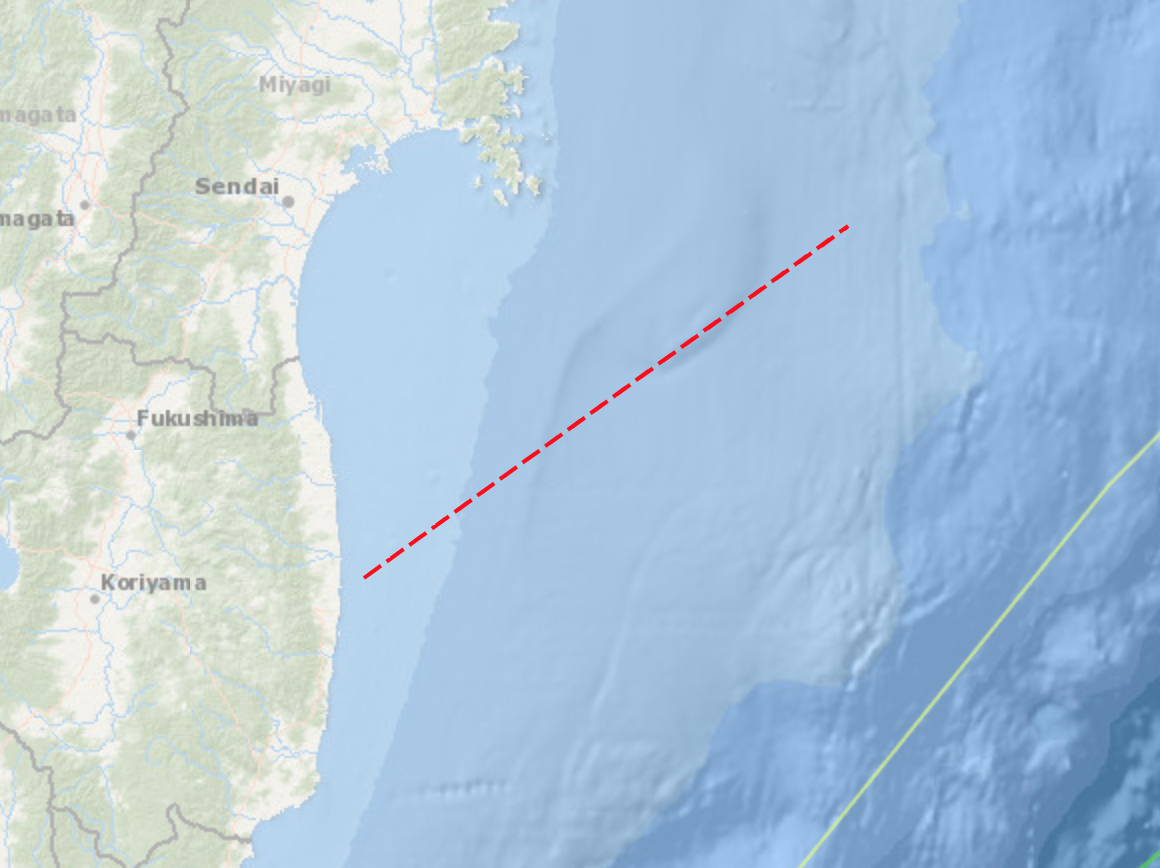
\includegraphics[scale=0.5]{1D.png}
\end{figure}
\noindent Using the control points, we can then apply the cubic B\'ezier curve to derive the following sea floor curve:
\begin{figure}[H]
\centering
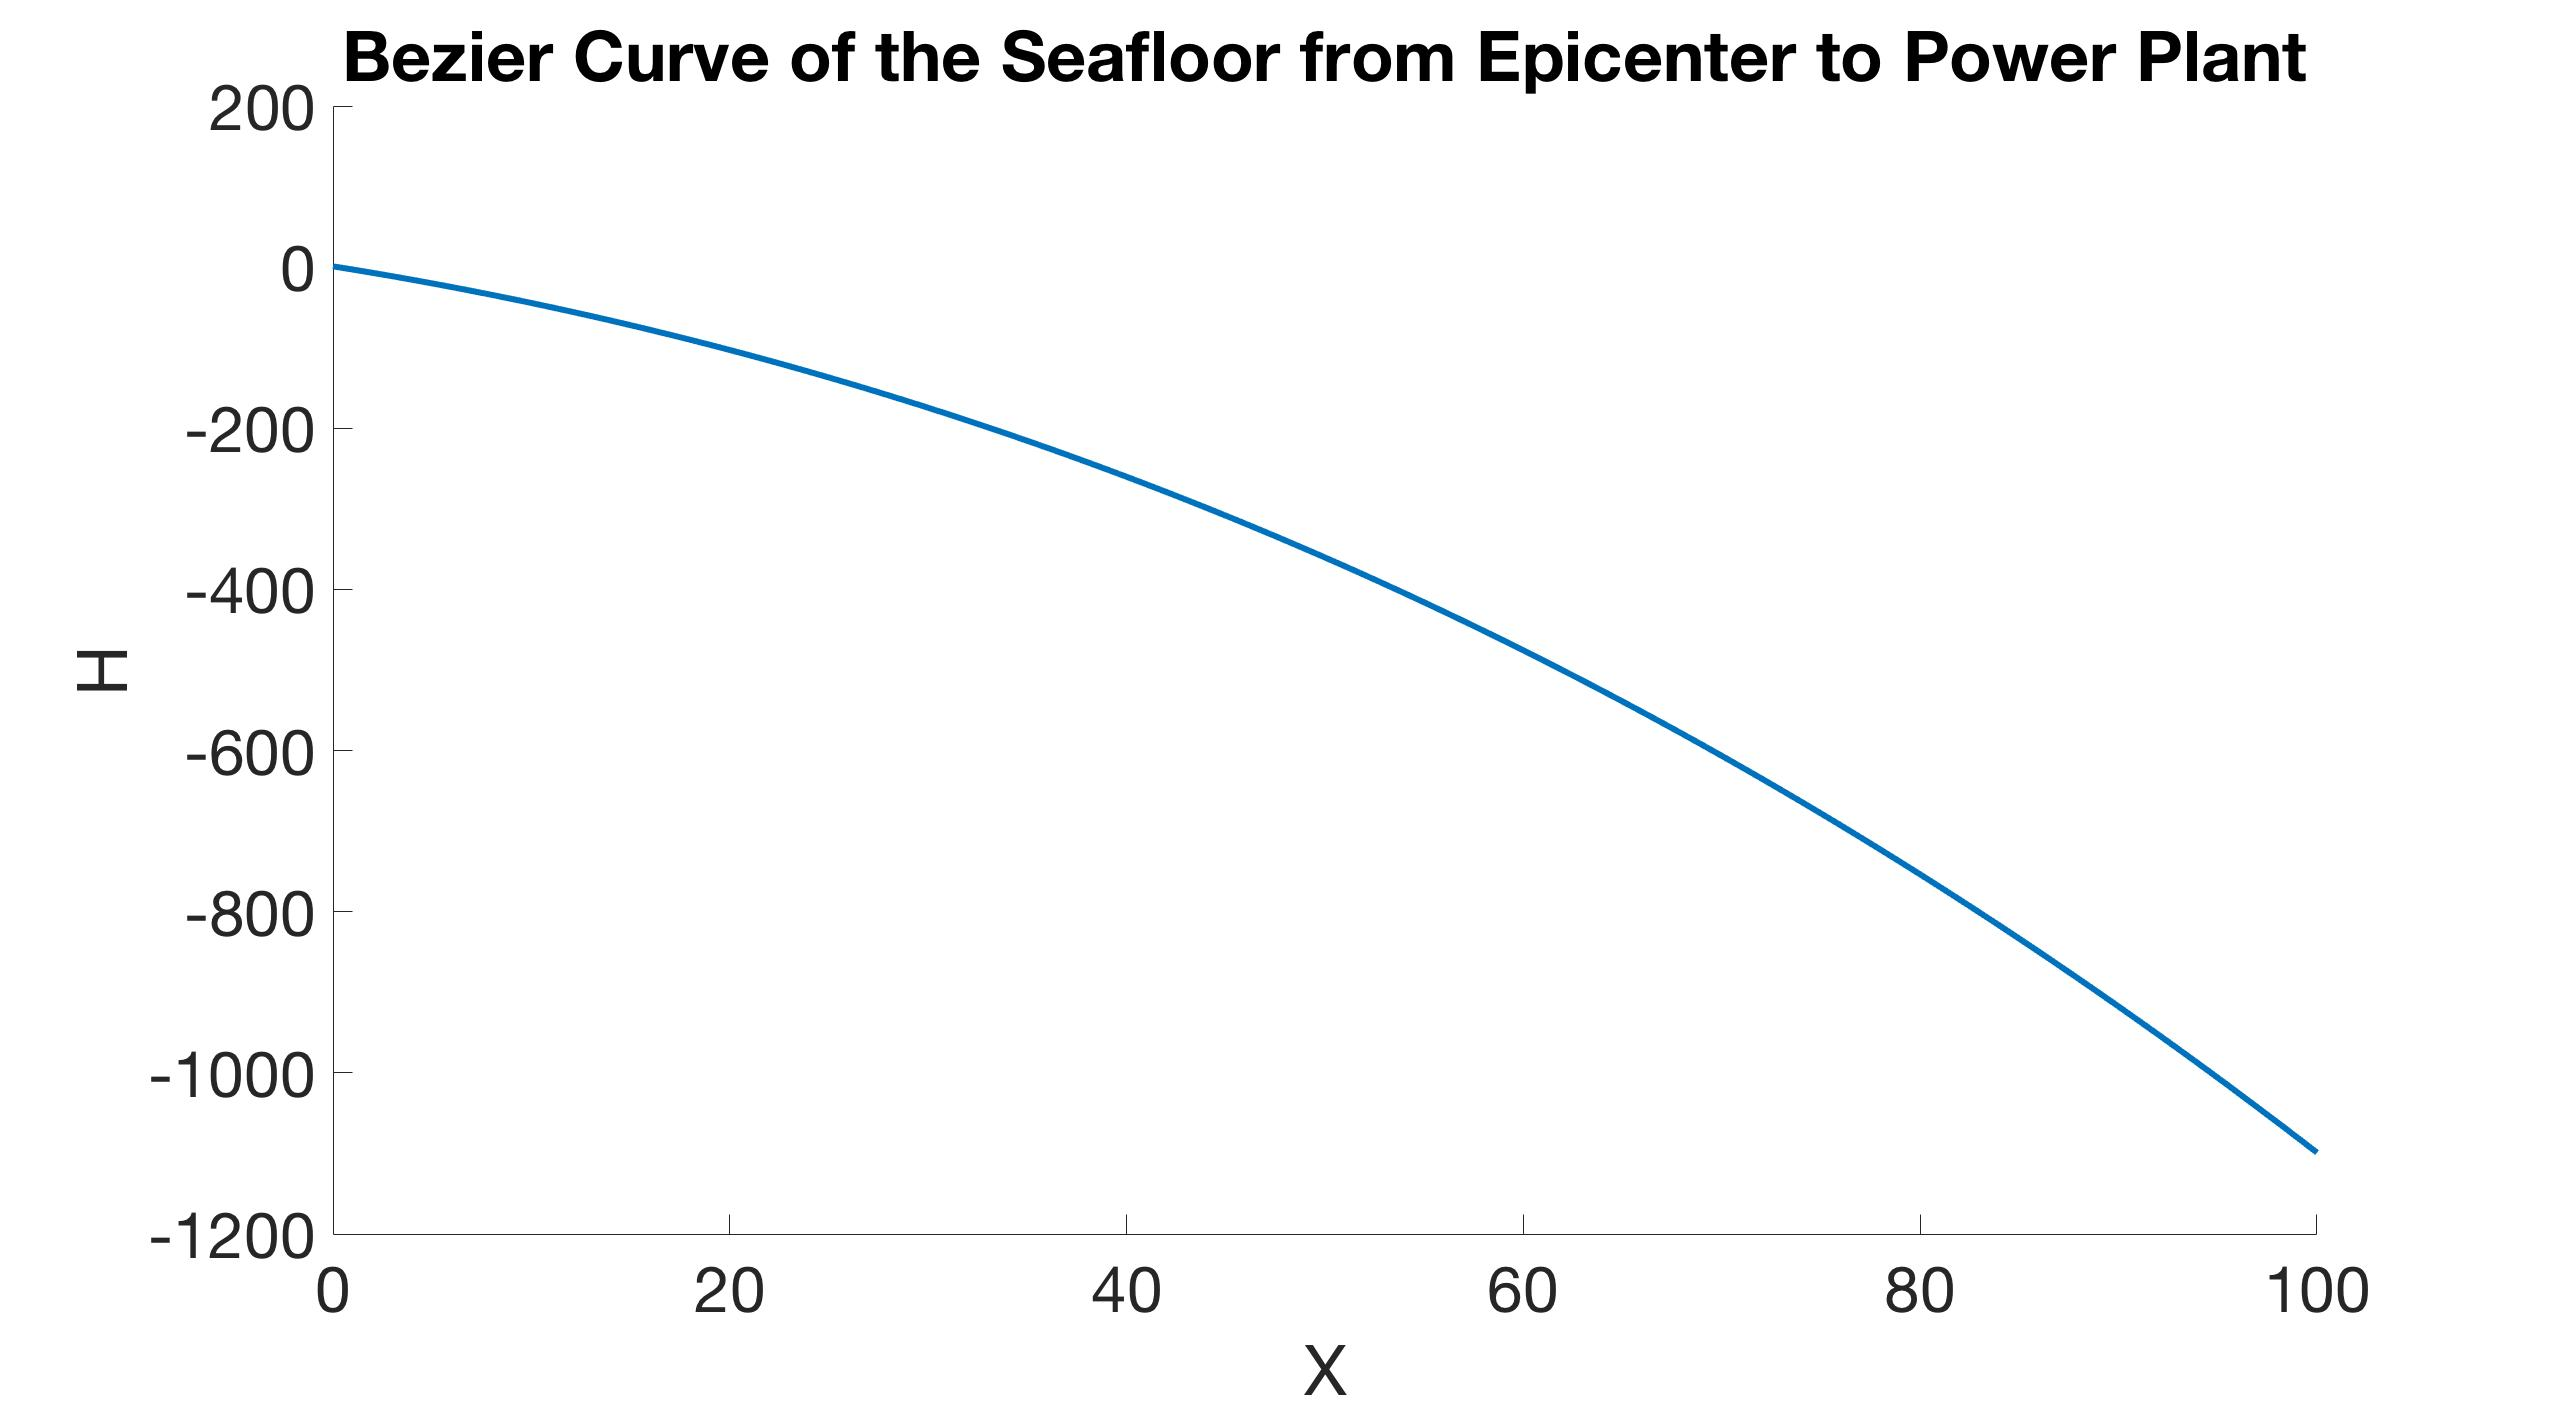
\includegraphics[scale=0.15]{1DLine.jpg}
\end{figure}
\begin{figure}[H]
\centering
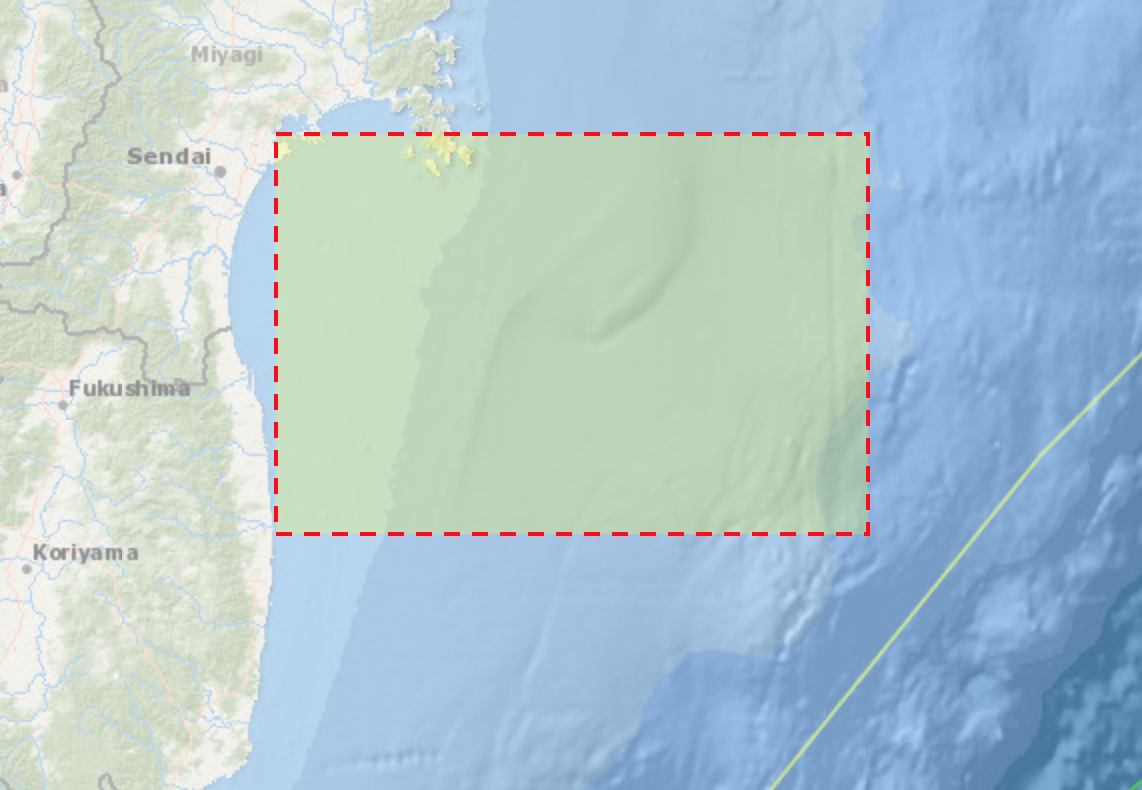
\includegraphics[scale=0.5]{2D.png}
\end{figure}
\noindent Using the control points, we can then apply the cubic B\'ezier curve to derive the following sea floor curve:
\begin{figure}[H]
\centering
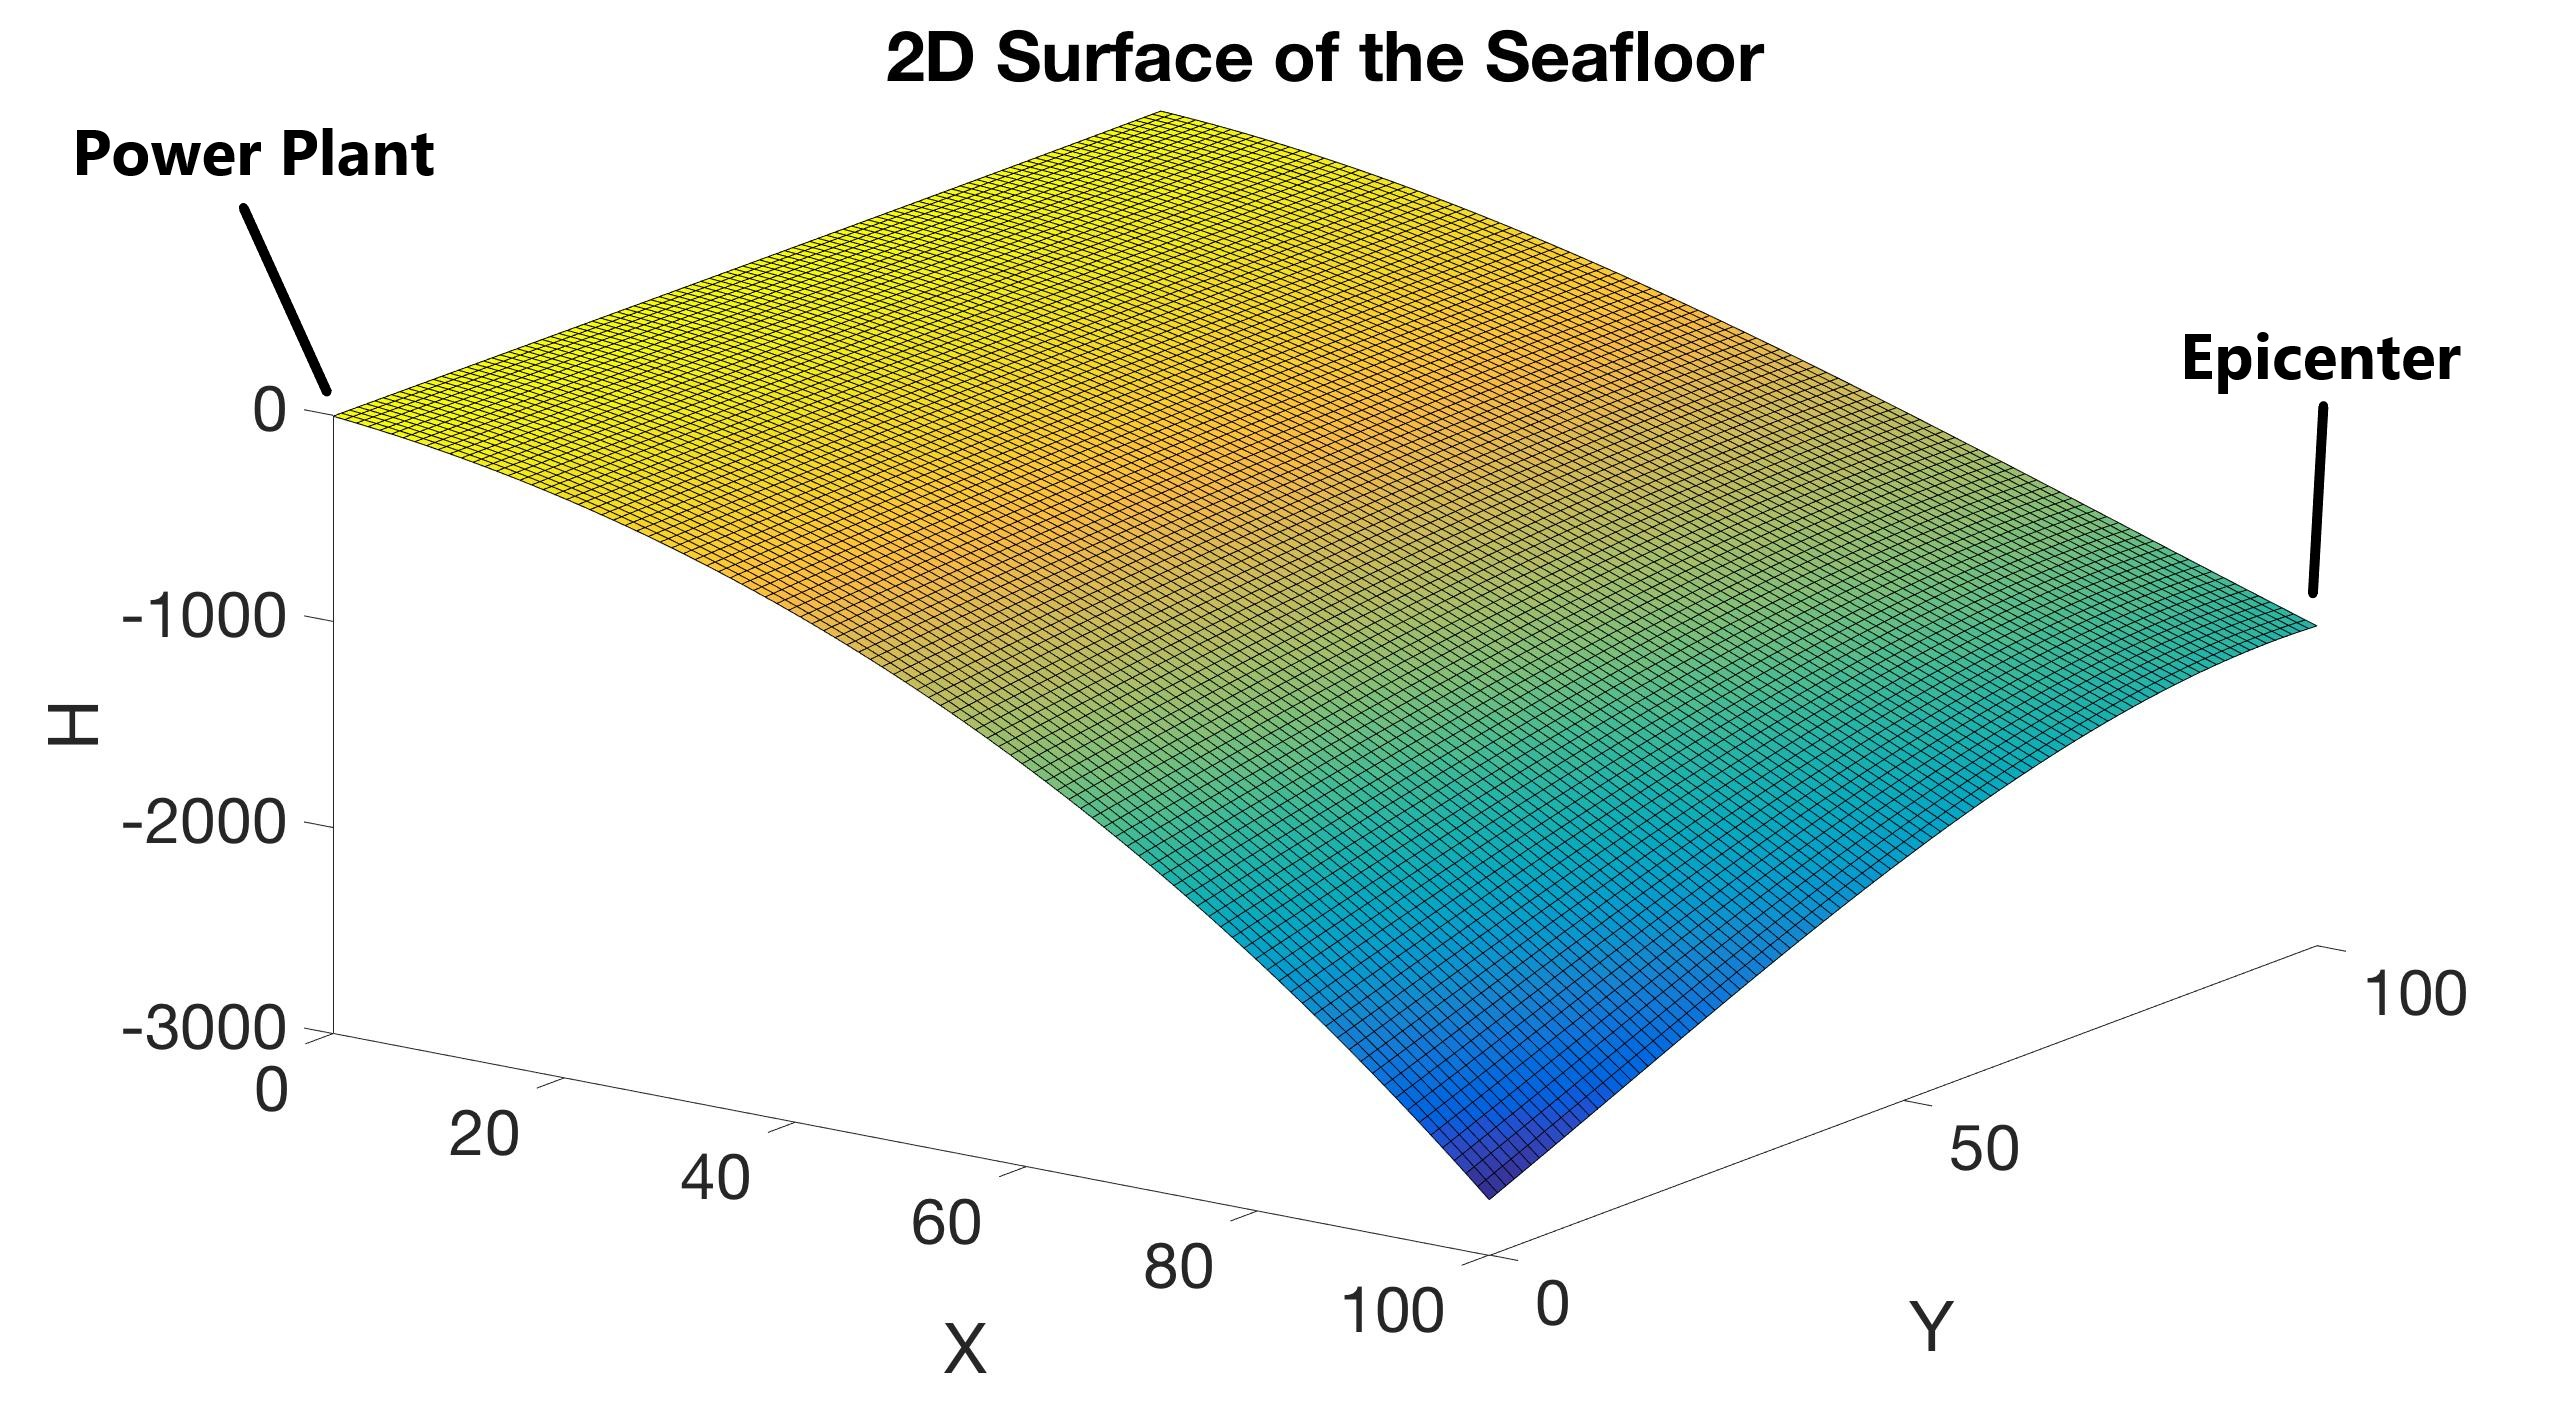
\includegraphics[scale=0.15]{2DSurf.jpg}
\end{figure}

\end{document}
